
\documentclass[12pt]{article}
\usepackage[utf8]{inputenc}
\usepackage[T1]{fontenc}
\usepackage{amsmath}

\usepackage{amssymb}
\usepackage{amsmath}
%\usepackage{amsthm}
\usepackage{amsopn}
\usepackage{graphicx}
\usepackage{mathrsfs}
\usepackage{empheq}

\usepackage{tikz}
\usetikzlibrary{fit,positioning}
\usetikzlibrary{arrows}

%\usepackage{showkeys}



%\setlength{\arraycolsep}{2pt}
%\setlength{\parskip}{.04in}
%\setlength{\footskip}{30pt}

\let\bb\mathbb       % BlackBoardBold (double letters)

\def\1{\mathbf 1}

  \def\AA{{\bb A}}\def\CC{{\bb C}}\def\DD{{\bb D}}\def\EE{{\bb E}}
  \def\GG{{\bb G}}\def\HH{{\bb H}}\def\KK{{\bb K}}\def\LL{{\bb L}}
  \def\MM{{\bb M}}\def\QQ{{\bb Q}}\def\TT{{\bb T}}\def\YY{{\bb Y}}
  \def\PP{{\bb P}}\def\II{{\bb I}}\def\WW{{\bb W}}\def\XX{{\bb X}}
  \def\VV{{\bb V}}\def\SS{{\bb S}}\def\BB{{\bb B}}\def\NN{{\bb N}}
  \def\RR{{\bb R}}\def\ZZ{{\bb Z}}\def\FF{{\bb F}}\def\DD{{\bb D}}
  \def\OO{{\bb O}}\def\JJ{{\bb J}}\def\UU{{\bb U}}

\def\cH{\mathcal H}
\def\cY{\mathcal Y}
\def\cX{\mathcal X}
\def\cA{\mathcal A}
\def\mC{\mathcal C}
\def\Ex{\mathbf E}

\def\bb{\mathbb}
%end of header
\def\hat{\widehat}
\def\bfX{\mathbf X}
\def\bfB{\mathbf B}
\def\bSigma{\boldsymbol\Sigma}
\def\bOmega{\boldsymbol\Omega}
\def\bmu{\boldsymbol\mu}
\def\bnu{\boldsymbol\nu}
\def\bPi{\boldsymbol\Pi}
\def\bX{\boldsymbol X}
\def\bx{\boldsymbol x}

\def\ci{\perp\!\!\!\perp}

\parskip=3pt
\renewcommand{\baselinestretch}{1.08}

\title{\vspace{-60pt}~\\Double sparsity in high-dimensional Gaussian mixture estimation and clustering\\Subject Overview}
\author{\vspace{-20pt}~\\ Laboratory Supervisor: A.S. Dalalyan\\
PHd Student: M. Sebbar}
\date{\today}

\begin{document}
\maketitle
\tableofcontents
\newpage
\section{Introduction}
The broad goal of this thesis is to tackle a clustering problem in the scope of mixtures model framework. More precisely, we will study the clustering of points drawn from high-dimensional Gaussian mixtures distributions.\\Thus, in the first part of this section we study the gaussian mixture model and the second part we describe the well know algorithm Expectation-Maximization (EM) and the limitations in high-dimensional setting.
\subsection{The Gaussian mixture model}

The Gaussian mixture model is an important framework where the components are Gaussian distributions with parameters $(\mu_i,\Sigma_i)$. The distribution is given by:
\begin{equation}
p(x|\theta)=\sum_{i=1}^K\pi_i\frac{1}{(2\pi)^{d/2}|\Sigma_i|^{1/2}} e^{-\frac{1}{2}(x-\mu_i)^T\Sigma_i^{-1}(x-\mu_i)}=\sum_{i=1}^K\pi_i\mathcal N(x|\mu_i,\Sigma_i)
\end{equation}
with $\theta=\{\mu_1,\dots,\mu_K,\Sigma_1,\dots,\Sigma_K\}$ and $\forall i, \pi_i>0$ and $\sum_{i=1}^K\pi_i=1$
\\

We will study this mixture from a latent variable perspective. Let Z be a multionomial random variable with component $Z^i$, we have:
\begin{equation}
p(x|\theta)=\sum_{i=1}^K p(Z^i=1)p(x|Z^i=1,\theta)
\end{equation}
Therefore $\pi_i=p(Z^i=1)$ and reflects the probability that x is drawn from the $i^{th}$ mixture component.\\

In the clustering problem, we would like to calculate the probability of the latent variable Z conditioned on X in order to assign X to a cluster.\\
We denote $\tau^k=p(Z^k=1|x,\theta)$, from Bayes's rule we have:

\begin{equation}
\label{tau_bayes}
\tau^k=\frac{p(x|Z^k=1,\theta)p(Z^k=1)}{p(x|\theta)}=\frac{\pi_k \mathcal N(x|\mu_k,\Sigma_k)}{\sum_{i=1}^K\pi_i\mathcal N(x|\mu_i,\Sigma_i)}
\end{equation}

where $\pi_i=P(Z^i=1)$ the prior probability and $\tau^i$ the posterior.\\

We would like to estimate $\theta$ from a set of iid observations $X_1,\dots,X_N$ with $X_i\in \RR^d$. The related graphical model is:

%%GRAPH of pgm
\begin{figure}[h]
\centering
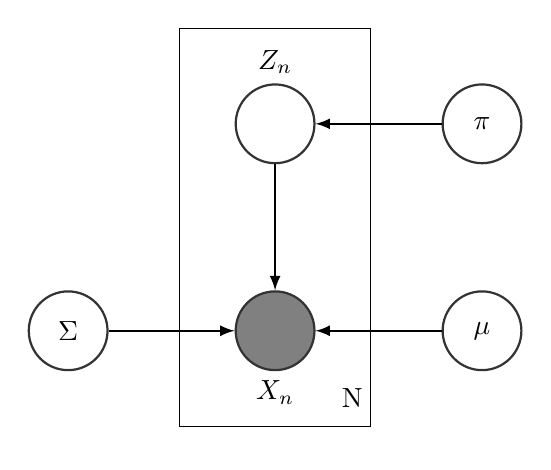
\begin{tikzpicture}
\tikzstyle{main}=[circle, minimum size = 10mm, thick, draw =black!80, node distance = 16mm]

\tikzstyle{connect}=[-latex, thick]
\tikzstyle{box}=[rectangle, draw=black!100]
  \node[main, fill = black!50] (x) [label=below:{$X_n$}] { };
  \node[main] (z) [above=of x,label=above:{$Z_n$}] {};

  \path (z) edge [connect] (x);

  \node[rectangle, inner sep=7mm,draw=black!100, fit= (z) (x)] {};
\node[rectangle, below=of x, inner sep=-10mm, fit= (z) (x),label=below right:N, xshift=7mm,yshift=-9mm] {};

\node[main] (a) [right=of x] {$\mu$};
\path (a) edge [connect] (x);
\node[main] (b) [left=of x] {$\Sigma$};
\path (b) edge [connect] (x);
\node[main] (c) [right=of z] {$\pi$};
\path (c) edge [connect] (z);
\end{tikzpicture}
\end{figure}

The log-likelihood is:

\begin{equation}
l(\theta|D)=\sum_{n=1}^{N}\log{p(x_n|\theta)}=\sum_{n=1}^{N}\log{\sum_{i=1}^K\pi_i\mathcal N(x_n|\mu_i,\Sigma_i)}
\end{equation}

Where D is the set of data points. Here we have the log of a sum and the maximization of the log-likelihood is a non-linear problem (contrary to exponential family distributions where the log acts on a simple probability distribution and therefore yields simple expressions).\\
An approach for the estimation of the maximum of log-likelihood is the Expectation-Maximization Algorithm.

%%%%%%%%%%%%%%%%%%%

\subsection{The EM Algorithm}

We will infer the values of $\{z_n\}$ conditioned to the data $\{x_n\}$. A natural approach to estimate the parameters $\theta$ is to estimate the mean of each class by deriving the log-likelihood with respect to $\mu_k$ and setting to 0 we have:


\begin{equation}
\sum_{n=1}^N\frac{\pi_k \mathcal N(x_n|\mu_k,\Sigma_k)}{\sum_{i=1}^K\pi_i\mathcal N(x_n|\mu_i,\Sigma_i)} \Sigma_k(x_n-\mu_k)=\sum_{n=1}^N \tau_n^k \Sigma_k(x_n-\mu_k)=0
\end{equation}
Assuming that $\Sigma_k$ is non singular, we have:

\begin{equation}
\mu_k=\frac{\sum_{n=1}^N\tau_n^k x_n}{\sum_{n=1}^N\tau_n^k}
\end{equation}

Doing a similar calculus for $\Sigma_k$, we have:

\begin{equation}
\Sigma_k=\frac{\sum_{n=1}^N \tau_n^k (x_n-\mu_k)(x_n-\mu_k)^T}{\sum_{n=1}^N\tau_n^k}
\end{equation}

Finally, maximizing the log-likelihood with respect to $\pi_k$ with the condition $\sum_{k=1}^K\pi_k=1$ (using Lagrange multiplier), we have:
\begin{equation}
\pi_k=\frac{\sum_{n=1}^N\tau_n^k}{N}
\end{equation}

However, as seen in \eqref{tau_bayes}, $\tau_n^k$ depends on the parameter estimates which depends on $\tau_n^k$. An idea would be to initialize the parameters and iterate. We calculate the posterior probability and then estimate the parameter $\theta$. This is the idea of the EM algorithm.
\\

\subsubsection{The EM algorithm for Gaussian Mixtures:}
\begin{enumerate}
\item[0.] Initialize parameters $\mu_k^0,\; \Sigma_k^0,\;\pi_k^0$
\item Calculate (Expectation Step):
\begin{equation}
\tau_n^{k,(t+1)}=\frac{\pi_k^{(t)} \mathcal N(x_n|\mu_k^{(t)},\Sigma_k^{(t)})}{\sum_{i=1}^K\pi_i^{(t)}\mathcal N(x_n|\mu_i^{(t)},\Sigma_i^{(t)})}
\end{equation}
\item Calculate (Maximization Step):
\begin{itemize}
\item
\begin{equation}
\mu_k^{(t+1)}=\frac{\sum_{n=1}^N\tau_n^{k,(t+1)} x_n}{\sum_{n=1}^N\tau_n^{k,(t+1)}}
\end{equation}
\item
\begin{equation}
\Sigma_k^{(t+1)}=\frac{\sum_{n=1}^N \tau_n^{k,(t+1)} (x_n-\mu_k^{(t+1)})(x_n-\mu_k^{(t+1)})^T}{\sum_{n=1}^N\tau_n^{(t+1)}}
\end{equation}
\item
\begin{equation}
\pi_k^{(t+1)}=\frac{\sum_{n=1}^N\tau_n^{(t+1)}}{N}
\end{equation}
\end{itemize}
\item Evaluate the log-likelihhod and check for convergence
\end{enumerate}

\subsubsection{Limitations of the EM Algorithm:}

EM is conceptualy easy and each iteration improves $l(\theta)$. However, the complexity of EM algorithm is $O(dn+Kn^2)$ and it requires many iterations. Unfortunately, in our case, the algorithm slows down in the high dimensional setting. We hope to tackle this probnlem by making sparsity assumptions on the structure of the precision matrix $\Sigma^{-1}$.

%%%%%%%%%%%%%%%%%%%%%%
\section{A structural analysis on $\bSigma$ approach}

We consider a multivariate Gaussian distribution with mean $\bmu^*$ and covariance $\bSigma^*$ and $Y_1,\dots,Y_N \in \RR^p$ iid drawn from this distribution. We would like to estimate $\bmu^*$ and $\bSigma^*$. We know that $\hat\bmu_n=\bar Y_n$, then WLOG we consider $\mu^*=0$, the problem is to estimate $\bSigma^*$. We will study the precision matrix and consider that $\Sigma^{-1}$ is sparse. We note $\Sigma^{-1}=\Omega$.\\
If $\Sigma^{-1}_{ij}=0 \Rightarrow Y_i \ci Y_j$ conditionnaly to $Y_{l\ne\{i,j\}}$. Thus, it makes sense to impose a $L_1$ penalty on $\Sigma^{-1}$ to increase its sparsity.

\subsection{Graphical Lasso}
\begin{equation}
\mathcal N(x|\mu^*,\Sigma^*)
=\frac{1}{(2\pi)^{d/2}|\Sigma^*|^{1/2}}\exp^{-\frac{1}{2}(x-\mu^*)^T\Sigma^{-1*}(x-\mu^*)}
\end{equation}
The log-likelihood, with $\mu=0$ is given by:
\begin{equation}
\mathcal{L}(\Sigma)=\log\left(\prod_{n=1}^N\frac{1}{(2\pi)^{d/2}|\Sigma|^{1/2}}\exp^{-\frac{1}{2}(x_n)^T\Sigma^{-1}(x_n)}\right)
\end{equation}
\# write eqs\\
\\
\begin{equation}
L(\Sigma)=C
+\frac{N}{2}\log|\Sigma^{-1}|-\frac{1}{2} tr(S_n\Sigma^{-1})
\end{equation}
Thus, considering the sparsity of $\Omega$, we impose a penalization to the maximum likelihood estimator of $\Sigma^{-1}$
\begin{equation}
\hat\Omega\in argmin\left\{ \log(|\Omega|)-tr(S_n\Omega)-\lambda||\Omega||_1   \right\}
\end{equation}
A reason to use the $L_1$ penalization instead of the ridge is that for an $L_p$ penalization, the prpblem is convex for $p\geq 1$ and we have parsimonious property for $p\leq 1$.
\subsection{Column-Wise Lasso}
\section{Comments}
\section{References}

\end{document}
